% Chapter 2: Literature Review 
\chapter{Literature Review}
\label{ch:literature}

\section{Causal Inference Methods in Finance}
Financial economists have created several methods to find causality from data that is not from an experiment. Foundational methods like \textbf{Difference-in-Differences (DiD)} and \textbf{matching methods} attempt to replicate the conditions of a randomized experiment using observational data. This section reviews these established techniques, discusses their connection to Optimal Transport (OT), and introduces the modern causal discovery algorithms that form the core of this thesis.

\subsection*{Difference-in-Differences and Changes-in-Changes}
DiD is a widely used method in finance for estimating the causal impact of specific events or policies \cite{Athey16}. It compares the change in outcomes over time between a \textit{treated} group and an untreated \textit{control} group. By differencing out common time trends and fixed group differences, DiD aims to isolate the treatment effect under the key assumption of \textit{parallel trends}. This assumption states that both groups would have evolved similarly in the absence of the treatment. While standard DiD focuses on average effects, extensions like \textit{Changes-in-Changes (CiC)} by Athey and Imbens generalize the approach to capture effects across the entire distribution \cite{Athey06}. More recently, optimal transport has been proposed to create a distributional version of DiD, which can measure how the entire shape of the return distribution shifts due to a treatment, a concept particularly relevant for financial risk analysis \cite{Torous24}.

\subsection*{Matching Methods and Propensity Scores}
Matching methods offer another way to control for confounding by constructing a control group that is statistically similar to the treated group based on observed characteristics. A common approach is \textbf{propensity score matching (PSM)}, where units are matched based on their probability of receiving treatment \cite{Rosenbaum83}. However, finding good matches can be difficult in high-dimensional settings. \textbf{Optimal Transport} provides a powerful alternative by re-weighting the entire control group to make its covariate distribution as close as possible to the treated group's distribution \cite{Torous24}. This distributional matching often leads to better balance and more reliable causal estimates than traditional one-to-one matching.

\subsection*{Instrumental Variables}
The \textbf{Instrumental Variables (IV)} approach is a classic econometric method for dealing with confounding when there is an unobserved variable that affects both the treatment and the outcome. IV relies on finding an "instrument" that is correlated with the treatment but does not affect the outcome directly, except through the treatment variable. While powerful in theory, finding a truly valid instrument that satisfies these conditions is notoriously difficult in complex financial markets, where variables are highly interconnected.

\subsection*{The Peter-Clark (PC) Algorithm}
Constraint-based algorithms represent a foundational approach to causal discovery. The most well-known of these is the \textbf{Peter-Clark (PC) algorithm}, named after its creators Peter Spirtes and Clark Glymour \cite{Spirtes00}. The PC algorithm operates by starting with a fully connected undirected graph and then systematically removes edges between variables based on conditional independence tests. By iteratively testing for independence conditioned on different sets of variables, it identifies the underlying causal "skeleton." In the final step, it applies orientation rules to determine the direction of some of the edges, resulting in a causal graph that represents the conditional independence relationships in the data.

\subsection*{OT for Causal Direction (DIVOT)}
Finding the direction of causality between two variables is a hard problem. \textbf{Tu et al. (2022)} created a method called \textit{DIVOT (Distributional Inference of Variable Order with Transport)} that uses optimal transport for this task\cite{Tu22}. The method is based on the idea of a \textit{functional causal model}. If X causes Y, then the distribution of Y can be seen as the distribution of X moved by some function. DIVOT calculates the OT map from X to Y and from Y to X. It then checks which map is more plausible. In simple terms, if X causes Y, it should be "cheaper" to transport the distribution of X to match Y than the other way around.

In our factor investing world, DIVOT could help us understand if volatility drives returns, or if returns drive volatility. This is an old debate. An OT based test could give us evidence for one direction over the other by looking at how the distributions of these variables move into each other.

\subsection*{OT for Counterfactuals and Distributional Robustness}
Another related idea is using OT to estimate counterfactuals. \textbf{Charpentier et al. (2023)} show that OT can create counterfactuals for individual units\cite{Charpentier23}. It does this by transporting an observation in the treated group to a similar observation in the control group. In finance, we could ask "What would this stock's return have been if it was not exposed to the momentum factor?". OT can help answer this by finding a "nearest" stock in the unexposed group and adjusting for the differences in the distributions.

OT also gives us a tool to check for robustness. In finance, market regimes can change, and this can break causal links. By modeling changes in distributions directly, OT based methods might be less sensitive to these changes. This makes them good for factor investing.

\section{Mathematical Foundations and Key Definitions}

To ensure clarity and ease of understanding, we provide formal definitions of key mathematical concepts used throughout this thesis.

\subsection*{Optimal Transport}
\textbf{Optimal Transport (OT)} is the mathematical framework that solves the problem of moving mass from one distribution to another at minimal cost. Given two measures $\mu$ and $\nu$, OT finds the transport plan $\pi^*$ that minimizes the total transportation cost:

\[
\pi^* = \arg\min_{\pi \in \Pi(\mu, \nu)} \int c(x, y) \, d\pi(x, y)
\]

where $c(x, y)$ is the cost function for moving mass from point $x$ to point $y$.

\textbf{Application in causal inference}: We use OT in our DIVOT algorithm to compare the cost of mapping a factor's distribution to the return's distribution, and vice-versa, to infer the causal direction.

\subsection*{Wasserstein Distance}
The \textbf{Wasserstein distance} (also known as the Earth Mover's Distance) is a measure of the distance between two probability distributions, derived from the optimal transport cost. For two probability measures $\mu$ and $\nu$ on a metric space $(M, d)$, the 2-Wasserstein distance is defined as the square root of the minimal transport cost when the cost function is the squared distance:

\[
W_2(\mu, \nu) = \left(\inf_{\pi \in \Pi(\mu, \nu)} \int_{M \times M} d(x, y)^2 \, d\pi(x, y)\right)^{1/2}
\]

where $\Pi(\mu, \nu)$ is the set of all joint probability measures on $M \times M$ with marginals $\mu$ and $\nu$, and $d(x, y)$ is the distance between points $x$ and $y$.

\textbf{Implementation details}: We compute Wasserstein distances using the \textbf{Python Optimal Transport (POT) library}\cite{Flamary21}, specifically the \texttt{ot.emd2()} function.

\textbf{Why we use it}: In our DIVOT method, we use the Wasserstein distance as a key metric to quantify the "cost" of transforming one distribution into another, which helps us determine the most likely causal direction.

\section{Recent Developments in Causal Analysis}
Our work is also informed by broader advances in econometrics and causal inference in the social sciences. \textbf{Athey and Imbens (2016)} survey the "state of applied econometrics" and emphasise credible design and validation techniques for causal studies\cite{Athey16}. They highlight recent innovations such as synthetic control methods and rigorous robustness checks (placebo tests, sensitivity analyses) as essential tools for empirical researchers.

\textbf{Imbens (2024)} provides another perspective, focusing on the integration of machine learning with causal inference and the challenges of big data\cite{Imbens24}. He notes that while classical methods have solid theoretical foundations, newer techniques can handle more complex scenarios. In factor investing, the availability of rich datasets means methods that can exploit more data and capture nonlinear patterns, without sacrificing rigor, are valuable. A key motivation for employing these sophisticated methods is the prevalence of specification errors in financial models that can lead to "factor mirages." As López de Prado explains, two critical risks are \textbf{confounder bias} and \textbf{collider bias} \cite{LopezDePrado25}. Confounder bias arises when a variable influences both the factor and the return, creating a spurious correlation if not controlled for. Collider bias is more subtle; it occurs when a researcher conditions on a variable that is a common effect of both the factor and the outcome, which can artificially induce a correlation between them where none exists. Understanding and mitigating these biases is essential for robust causal inference.

In summary, the literature suggests that combining established causal inference frameworks with modern computational techniques (such as OT) shows potential. This thesis builds on these ideas, aiming to show that such a combination can indeed move factor investing research toward robust, causally grounded insights. By designing our simulation and choice of methods based on previous research, we ensure that our approach is not only novel but also rooted in the best practices and lessons learned from prior work.

\begin{figure}[ht]
\centering
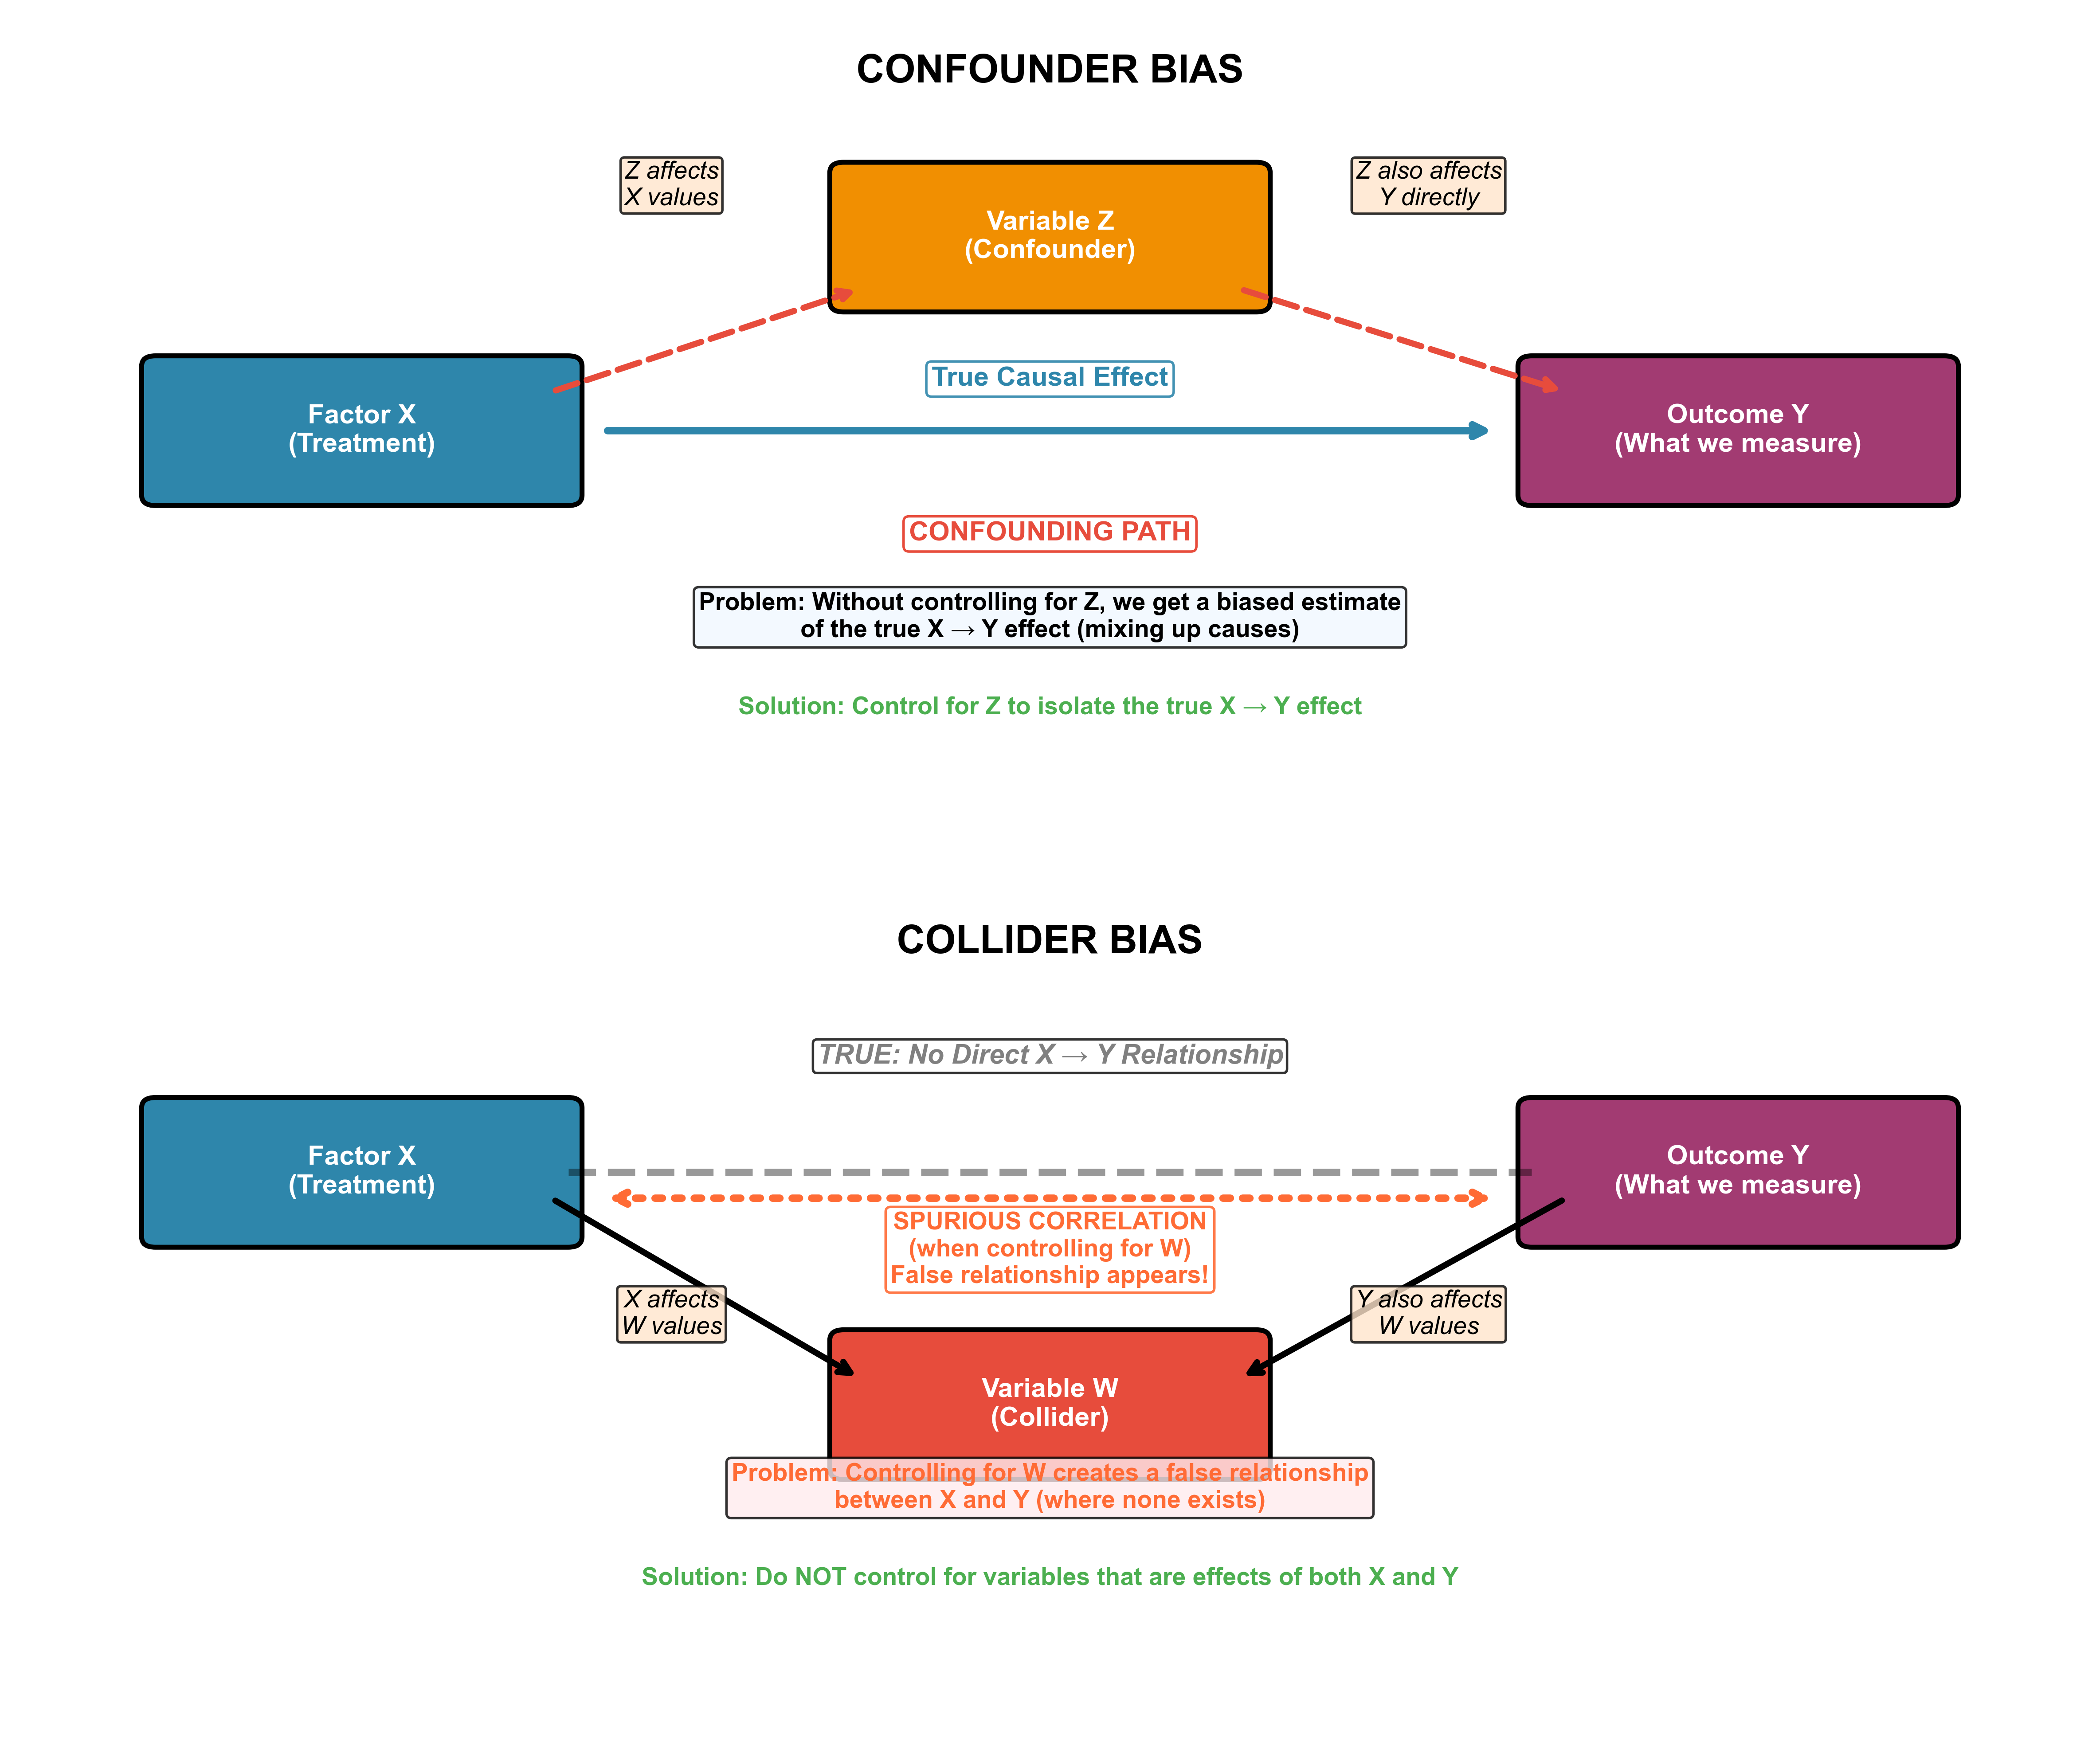
\includegraphics[width=0.85\textwidth]{Graphs/Synthetic/confounder_collider_bias_explanation.png}
\caption{Confounder and Collider Bias in Causal Inference. Illustration of two fundamental sources of bias in causal analysis. Top panel: Confounder bias occurs when variable Z affects both treatment X and outcome Y, creating a backdoor confounding path (dashed arrows) that biases causal estimates unless Z is controlled. Bottom panel: Collider bias arises when controlling for variable W, a common effect of both X and Y, which artificially induces a spurious correlation (dotted arrow) between X and Y where no true causal relationship exists. Proper causal inference requires controlling for confounders while avoiding control of colliders. Source: López de Prado (2023) \cite{Lopez23}.}
\label{fig:confounder_collider_bias}
\end{figure}